\begin{frame}
\frametitle{Положения, выносимые на защиту}
\begin{enumerate}
  \item Метод обучения с подкреплением, способный оперировать действиями различного масштаба и устойчивый к оптическим шумам. Разработанный метод позволяет настраивать оптический интерферометр без участия человека, основываясь исключительно на изображениях интерференционной картины. Предложенный метод не использует априорной информации и способен самостоятельно обучаться под конкретную установку.
  \item Программно-аппаратный комплекс автоматической настройки оптического интерферометра. Скорость и точность настройки с использованием разработанного метода существенно превосходят ручную настройку.
  \item Метод обучения стратегии для управления движением шагающего робота с заданной линейной и угловой скоростью.
  \item Иерархический алгоритм, комбинирующий алгоритмический и нейросетевой подходы. Алгоритм был протестирован в задаче управления агентом в среде NetHack.
    \end{enumerate}
\end{frame}
\note{
    Проговаривается вслух научная новизна
}

\begin{frame}
    \frametitle{Свидетельство о регистрации программы}
    \begin{figure}[h]
        \centering
        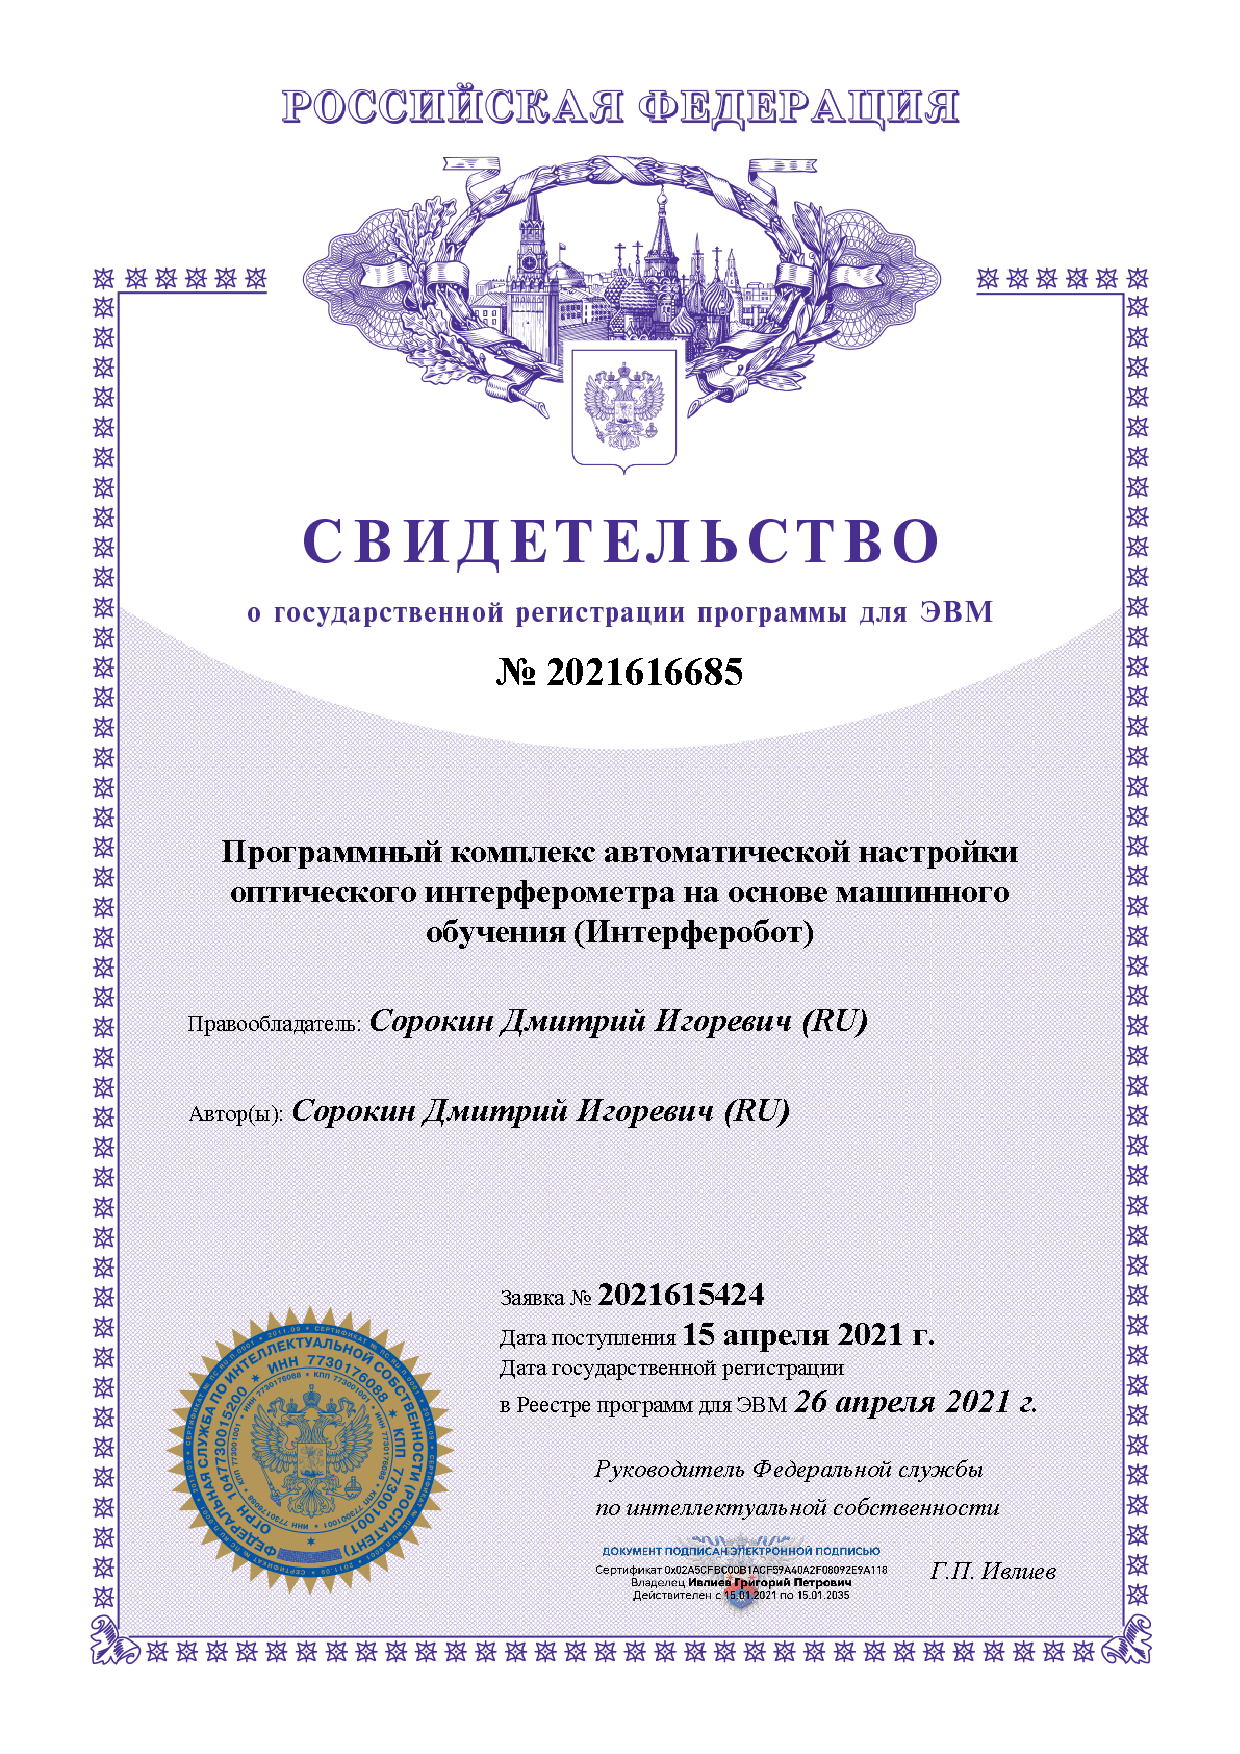
\includegraphics[height=0.7\textheight]{interferobot_rid.pdf}
    \end{figure}
\end{frame}
\note{
    Получено свидетельство о регистрации разработанной программы \textsc{Hello~world™}.
}

%\begin{frame}
%    \frametitle{Акт о внедрении}
%    \begin{figure}[h]
%        \centering
%        \fbox{
%            \begin{minipage}[t]{0.4\linewidth}
%                %\includegraphics[width=\linewidth]{implementation}
%            \end{minipage}
%        }
%    \end{figure}
%\end{frame}
%\note{
%    Получен акт о внедрении.
%}

%\begin{frame} % публикации на одной странице
\begin{frame}[t,allowframebreaks] % публикации на нескольких страницах
\frametitle{Публикации результатов диссертационной работы}

\begin{enumerate}
\fontsize{10pt}{10pt}\selectfont
    \item Interferobot: aligning an optical interferometer by a reinforcement learning agent. \textcolor{gray}{/. –– }\textbf{D. Sorokin}\textcolor{gray}{, A. Ulanov, E. Sazhina, A. Lvovsky // Advances in Neural Information Processing Systems. Vol. 33 / ed. by H. Larochelle, M. Ranzato, R. Hadsell, M. F. Balcan, H. Lin. –– Curran Associates, Inc., 2020. –– P. 13238––13248.} (CORE A*)
    \item Aligning an optical interferometer with beam divergence control and continuous action space. \textcolor{gray}{/. –– S. Makarenko,} \textbf{D. I. Sorokin}\textcolor{gray}{, A. Ulanov, A. Lvovsky // Proceedings of the 5th Conference on Robot Learning. Vol. 164 / ed. by A. Faust, D. Hsu, G. Neumann. –– PMLR, 2022. –– P. 918––927. –– (Proceedings of Machine Learning Research)}
    \item Insights From the NeurIPS 2021 NetHack Challenge. \textcolor{gray}{/. –– E. Hambro, S. Mohanty, D. Babaev, M. Byeon, D. Chakraborty, E. Grefenstette, M. Jiang, J. Daejin, A. Kanervisto, J. Kim, S. Kim, R. Kirk, V. Kurin, H. Küttler, T. Kwon, D. Lee, V. Mella, N. Nardelli, I. Nazarov, N. Ovsov, J. Holder, R. Raileanu, K. Ramanauskas, T. Rocktäschel, D. Rothermel, M. Samvelyan,} \textbf{D. Sorokin}\textcolor{gray}{, M. Sypetkowski, M. Sypetkowski // Proceedings of the NeurIPS 2021 Competitions and Demonstrations Track. Vol. 176 / ed. by D. Kiela, M. Ciccone, B. Caputo. –– PMLR, 2022. –– P. 41––52. –– (Proceedings of Machine Learning Research)} (CORE A*)
    \item Learning Various Locomotion Skills from Scratch with Deep Reinforcement Learning. \textcolor{gray}{/. –– }\textbf{D. I. Sorokin}\textcolor{gray}{, D. L. Babaev // Advances in Neural Computation, Machine Learning, and Cognitive Research VI / ed. by B. Kryzhanovsky, W. Dunin-Barkowski, V. Redko, Y. Tiumentsev. –– Cham : Springer International Publishing, 2023. –– P. 322––329.} (SCOPUS)
\end{enumerate}
    
\end{frame}
\note{
    Результаты работы опубликованы в N печатных изданиях,
    в~т.\:ч. M реферируемых изданиях.
}

\begin{frame}[t,allowframebreaks]
\frametitle{Презентации на международных конференциях}
\vspace{20pt}
\setlength{\leftmargini}{0cm}


\begin{columns}
\column{0.6\linewidth}

\begin{itemize}
\setlength\itemsep{1em}
    \item[] {\color{orange}Neural Information Processing Systems}\\
    NeurIPS 2020, (CORE A*)\\
    доклад был отмечен как spotlight
    \item[] {\color{orange}Conference on Robot Learning}\\
    CoRL 2021
    \item[] {\color{orange}Neural Information Processing Systems}\\
    NeurIPS 2021, (CORE A*)\\
    Competition track
    \item[] Международная научно-техническая конференция Нейроинформатика 2022 (SCOPUS)
\end{itemize} 
\column{0.4\linewidth}

\includegraphics[width=1\linewidth]{Presentation/images/logo/neurips.png}

\includegraphics[width=1\linewidth]{Presentation/images/logo/corl.png}

\includegraphics[width=1\linewidth]{Presentation/images/logo/neurips.png}

\includegraphics[width=1\linewidth]{Presentation/images/logo/neuroinfo.png}
\end{columns}

\begin{columns}
\column{0.7\linewidth}
\begin{itemize}
\vspace{40pt}
\setlength\itemsep{1.5em}
    \item[] Annual International Laser Physics Workshop\\
    LPHYS 2021
    \item[] International Conference on Quantum Technologies\\
    ICQT 2021
    \item[] Machine Learning Summer School\\
    MLSS 2019
\end{itemize} 

\column{0.3\linewidth}
\vspace{50pt}
\begin{itemize}
\setlength\itemsep{1.5em}
    \item[] {
\includegraphics[width=1\linewidth]{Presentation/images/logo/lphys.png}}
    \item[] {
\includegraphics[width=1\linewidth]{Presentation/images/logo/icqt.png}}
    \item[] {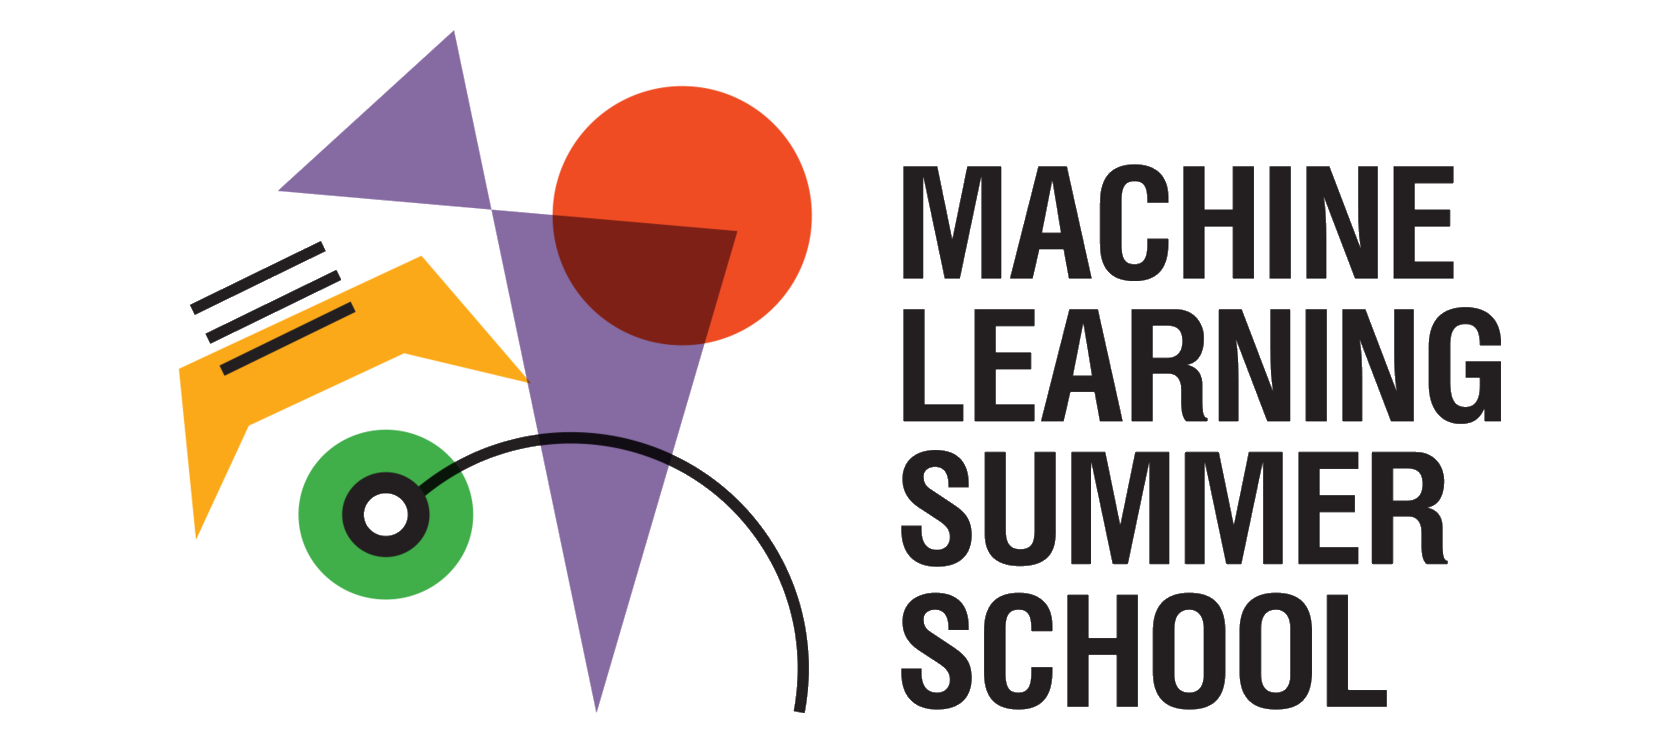
\includegraphics[width=1\linewidth]{Presentation/images/logo/mlss.png}}
\end{itemize}

\end{columns}

\end{frame}
\note{
    Работа была представлена на ряде конференций.
}

\begin{frame}[plain, noframenumbering] % последний слайд без оформления
    \begin{center}
        \Huge
        Спасибо за внимание!
    \end{center}
\end{frame}
